%% LyX 2.3.6.1 created this file.  For more info, see http://www.lyx.org/.
%% Do not edit unless you really know what you are doing.
\documentclass[english]{article}
\usepackage[T1]{fontenc}
\usepackage[latin9]{inputenc}
\usepackage{geometry}
\geometry{verbose,tmargin=2.5cm,bmargin=2.5cm,lmargin=2.5cm,rmargin=2.5cm}
\usepackage{calc}
\usepackage{textcomp}
\usepackage{graphicx}
\PassOptionsToPackage{normalem}{ulem}
\usepackage{ulem}

\makeatletter

%%%%%%%%%%%%%%%%%%%%%%%%%%%%%% LyX specific LaTeX commands.
%% Because html converters don't know tabularnewline
\providecommand{\tabularnewline}{\\}

%%%%%%%%%%%%%%%%%%%%%%%%%%%%%% User specified LaTeX commands.
\usepackage{soul}

\makeatother

\usepackage{babel}
\begin{document}
{[}SPLIT\_HERE{]}
\begin{enumerate}
\item \textbf{{[}HCI/PRELIM/9597/2015/P1/Q1{]} }

A program is to process the total points of football league teams
based on number of wins, draws and losses. The program can be run
every day. 

The program reads from file \texttt{TOP\_TEAM.txt} the current highest
points and team name from running the program on previous days. 

The program specification is to: 
\begin{itemize}
\item input \textbf{up to} four team names (max. 12 characters long) each
with the total number match wins, draws and losses so far.
\item calculate the total aggregate point for each team based on 3 points
for every win, 1 point for every draw and 0 points for every loss. 
\item display on screen: 
\begin{itemize}
\item the highest point with the team name for today 
\item a message saying whether or not the highest point today beat the current
team with the highest aggregate points. 
\end{itemize}
\item update the file \texttt{TOP\_TEAM.txt} if a higher aggregate point
was computed today. 
\end{itemize}

\subsection*{Task 1.1 }

Write program code for this task. 

\subsection*{Evidence 1: }

Your program code for Task 1.1. \hfill{}{[}8{]}

\subsection*{Task 1.2 }

Draw up a set of test data which tests the functioning of your program.
Consider carefully all cases which could occur for both the data input
and the two processing requirements. 

\subsection*{Evidence 2: }

A screenshot for each test case you considered. Annotate the screenshot
explaining the purpose of each test. \hfill{}{[}7{]}

{[}SPLIT\_HERE{]}
\item \textbf{{[}HCI/PRELIM/9597/2015/P1/Q2{]} }

The Russian peasant algorithm is an alternative method to perform
multiplication of whole numbers by consecutive application of doubling
numbers, halving numbers and addition. 

Consider the multiplication of \texttt{57} by \texttt{86} (= \texttt{4902}): 

Write each number side by side: 
\noindent \begin{center}
\texttt{\sout{57 ~~86}}
\par\end{center}

Double the first number and halve the second number (by performing
integer division by 2 i.e. drop the remainder).

If the second number or halving result is even, cross out this entire
row. Keep doubling, halving, and crossing out until the halving result
is 1.
\noindent \begin{center}
\noindent\begin{minipage}[t]{1\columnwidth}%
\texttt{\sout{57 ~~86}}

\texttt{\sout{114 ~43}}\texttt{ }

\texttt{\sout{228 ~21}}

\texttt{\sout{456 ~10}}

\texttt{\sout{912 ~5 }}

\texttt{\sout{1824 2 }}

\texttt{\sout{3648 1}}\texttt{ }%
\end{minipage}
\par\end{center}

Add up the remaining numbers in the first column. The total is the
product of the original numbers. 
\noindent \begin{center}
\noindent\begin{minipage}[t]{1\columnwidth}%
\texttt{~~~114}

\texttt{~~~228}

\texttt{~~~912}

\texttt{\uline{+ 3648 }}

\texttt{~~4902}%
\end{minipage}
\par\end{center}


\subsection*{Task 2.1 }

Write a function to implement the Russian peasant multiplication algorithm.
Test your function with the numbers \texttt{50} and \texttt{22}. 

\subsection*{Evidence 3: }

Your program code for Task 2.1. \hfill{} {[}7{]}

\subsection*{Evidence 4: }

Screenshot showing the output from running the program. \hfill{}
{[}1{]}

The Russian peasant algorithm is actually related to binary numbers.
Doubling a decimal number is to shift its binary equivalent left,
while halving a decimal number is to shift its binary equivalent right. 

Consider the multiplication of \texttt{13} by \texttt{12} (\texttt{=
156}) 

\noindent\begin{minipage}[t]{1\columnwidth}%
\texttt{~~~~}In Binary\texttt{ ~~~~~~~~~~~~~}In Decimal\texttt{ }

\texttt{~~~}\texttt{\sout{1101 1100}}\texttt{ ~~~~~~~~~~~}\texttt{\sout{13
12}}\texttt{ }

\texttt{~ }\texttt{\sout{11010 0110}}\texttt{ ~~~~~~~~~~~}\texttt{\sout{26
6}}\texttt{ }

\texttt{~110100 0011 ~~~~~~~~~~~52 3}

\texttt{1101000 0001 ~~~~~~~~~~104 1 }

\bigskip{}

\texttt{110100 + 1101000 = 10011100 = 156 (in decimal) }%
\end{minipage}

\subsection*{Task 2.2 }

Write a function \texttt{DecToBin()} to convert a decimal number to
its binary equivalent.

\subsection*{Evidence 5: }

Your program code for Task 2.2. \hfill{}{[}3{]}

\subsection*{Task 2.3}

Implement the Russian peasant multiplication algorithm using binary
numbers. Your program should accept 2 decimal numbers as input, convert
them to binary, and then perform the necessary operations to output
a binary string as the result. You should make use of your \texttt{DecToBin()}
function in Task 2.2. 

\subsection*{Evidence 6: }

Your program code for Task 2.3. \hfill{} {[}8{]}

\subsection*{Evidence 7: }

One screenshot showing the output from running the program code. \hfill{}
{[}1{]}

{[}SPLIT\_HERE{]}
\item \textbf{{[}HCI/PRELIM/9597/2015/P1/Q3{]} }

A message is encrypted and passed between two parties. To decrypt
the message, a \textquotedblleft key\textquotedblright{} is applied.
Both the sending and receiving parties hold the key which enables
them to encrypt and decrypt the message. 

An approach of cryptography is the simple substitution cipher, a method
of encryption by which each letter of a message is substituted with
another letter. The receiving party deciphers the text by performing
an inverse substitution. 

The substitution system is created by first writing out a \texttt{\emph{phrase}}.
The \texttt{\emph{key}} is then derived from the \texttt{\emph{phrase}}
by removing all the repeated letters. The \texttt{\emph{cipher text}}
alphabet is then constructed starting with the letters of the key
and then followed by all the remaining letters in the alphabet. 

Using this system, the phrase \textquotedbl\texttt{apple}\textquotedbl{}
gives us the \texttt{\emph{key}} as \textquotedbl\texttt{APLE}\textquotedbl{}
and the following substitution scheme: 

\begin{tabular}{lccccccccccccccccccccccccccc}
\textbf{Plain text alphabet:} & \texttt{a} & \texttt{b} & \texttt{c} & \texttt{d} & \texttt{e} & \texttt{f} & \texttt{g} & \texttt{h} & \texttt{i} & \texttt{j} & \texttt{k} & \texttt{l} & \texttt{m} & \texttt{n} & \texttt{o} & \texttt{p} & \texttt{q} & \texttt{r} & \texttt{s} & \texttt{t} & \texttt{u} & \texttt{v} & \texttt{w} & \texttt{x} & \texttt{y} & \texttt{z} & \tabularnewline
 & \texttt{$\downarrow$} &  &  & \texttt{$\downarrow$} &  &  &  &  &  &  &  &  &  &  &  &  &  &  &  &  &  &  &  &  &  & \texttt{$\downarrow$} & is substituted by\tabularnewline
\textbf{Cipher text alphabet:} & \texttt{A} & \texttt{P} & \texttt{L} & \texttt{E} & \texttt{B} & \texttt{C} & \texttt{D} & \texttt{F} & \texttt{G} & \texttt{H} & \texttt{I} & \texttt{J} & \texttt{K} & \texttt{M} & \texttt{N} & \texttt{O} & \texttt{Q} & \texttt{R} & \texttt{S} & \texttt{T} & \texttt{U} & \texttt{V} & \texttt{W} & \texttt{X} & \texttt{Y} & \texttt{Z} & \tabularnewline
\end{tabular}

\texttt{'a'} will be substituted by \texttt{'A'}, \texttt{'b'} will
be substituted by \texttt{'P'}, \texttt{'c'} will be substituted by
\texttt{'L'}, \texttt{'d'} will be substituted by \texttt{'E'}, \texttt{'e'}
will be substituted by \texttt{'B'}, and so on. 

\subsection*{Task 3.1 }

Write program code for a function to create cipher text using the
following specification: 
\noindent \begin{center}
\texttt{FUNCTION CreateCipher (phrase: STRING): STRING }
\par\end{center}

The function \texttt{CreateCipher} has a single parameter \texttt{phrase}
and returns the cipher text alphabet as a string. 

\subsection*{Evidence 8: }

Your program code for Task 3.1. \hfill{}{[}8{]}

\subsection*{Task 3.2 }

Write program code for a procedure \texttt{CreateCipherTest} which
does the following:
\begin{itemize}
\item read the phrases from file \texttt{PHRASES.txt} 
\item create cipher text for each of the phrases 
\item display each phrase and cipher text on the screen as follows: 

\noindent\fbox{\begin{minipage}[t]{1\columnwidth - 2\fboxsep - 2\fboxrule}%
\texttt{Phrase: apple}

\texttt{Cipher text: APLEBCDFGHIJKMNOQRSTUVWXYZ }

\texttt{... ... }

\texttt{... ... }%
\end{minipage}}
\end{itemize}

\subsection*{Evidence 9: }

Your program code for Task 3.2. \hfill{}{[}3{]}

\subsection*{Evidence 10: }

Screenshot for running Task 3.2.\hfill{} {[}1{]}

\subsection*{Task 3.3}

Write program code for a function to decrypt a message using the following
specification: 
\noindent \begin{center}
\texttt{FUNCTION Decrypt(enc\_message: STRING, cipher: STRING): STRING }
\par\end{center}

The function \texttt{Decrypt} accepts parameters \texttt{enc\_message}
and \texttt{cipher}, and returns the decrypted message as a string.
Parameter \texttt{enc\_message} is the encrypted message, and parameter
\texttt{cipher} is the cipher text alphabet.

\subsection*{Evidence 11: }

Your program code for Task 3.3.\hfill{} {[}6{]}

\subsection*{Task 3.4 }

Write program code which does the following: 
\begin{itemize}
\item read the phrase and encrypted message from file \texttt{CIPHER.txt}
\item cipher text is generated from \texttt{CreateCipher} function 
\item message is decrypted from \texttt{Decrypt} function
\item display decrypted message on the screen together with the phrase and
encrypted message 

\noindent\fbox{\begin{minipage}[t]{1\columnwidth - 2\fboxsep - 2\fboxrule}%
\texttt{Phrase: ... }

\texttt{Encrypted message: ... }

\texttt{Decrypted message: ...}%
\end{minipage}} 
\end{itemize}

\subsection*{Evidence 12: }

Your program code for Task 3.4. \hfill{}{[}3{]}

\subsection*{Evidence 13:}

Screenshot for running Task 3.4.\hfill{} {[}1{]}

\subsection*{Task 3.5 }

Write program code for a function to encrypt a message using the following
specification:
\noindent \begin{center}
\texttt{FUNCTION Encrypt(message: STRING, cipher: STRING): STRING }
\par\end{center}

The function Encrypt accepts parameters \texttt{message} and \texttt{cipher},
and returns the encrypted message as a string. Parameter \texttt{message}
is the message to be encrypted while parameter \texttt{cipher} is
the cipher text. 

\subsection*{Evidence 14: }

Your program code for Task 3.5. \hfill{}{[}4{]}

\subsection*{Task 3.6 }

Write program code which does the following: 
\begin{itemize}
\item encrypt the message: \textquotedbl\texttt{do not give up!}\textquotedbl{} 
\item use the phrase: \textquotedbl\texttt{skyhigh}\textquotedbl{} 
\item generate cipher text from \texttt{CreateCipher} function
\item message is encrypted using \texttt{Encrypt} function 
\item encrypted message is displayed on screen as follows: 

\noindent\fbox{\begin{minipage}[t]{1\columnwidth - 2\fboxsep - 2\fboxrule}%
\texttt{Phrase: skyhigh}

\texttt{Encrypted Message: ... }%
\end{minipage}}
\end{itemize}

\subsection*{Evidence 15: }

Your program code for Task 3.6. \hfill{} {[}3{]}

\subsection*{Evidence 16:}

Screenshot for running Task 3.6. \hfill{}{[}1{]}

{[}SPLIT\_HERE{]}
\item \textbf{{[}HCI/PRELIM/9597/2015/P1/Q4{]} }

The task is to store a dataset of students\textquoteright{} names
and test scores (max size of 20 students) as a binary tree structure.
The text file \texttt{s} stores the students\textquoteright{} names
and test scores in the following format:
\noindent \begin{center}
\texttt{<student Name>|<Score> }
\par\end{center}

All test scores are integer values in the range 0 to 100 inclusive. 

The program will use a user-defined type \texttt{Node} for each node
defined as follows: 
\begin{center}
\begin{tabular}{|l|l|l|}
\hline 
\texttt{\textbf{\hspace{0.01\columnwidth}}}\textbf{Identifier} & \texttt{\textbf{\hspace{0.01\columnwidth}}}\textbf{Data Type} & \texttt{\textbf{\hspace{0.05\columnwidth}}}\textbf{Description}\tabularnewline
\hline 
\texttt{LeftP} & \texttt{INTEGER} & The left pointer for the node\tabularnewline
\hline 
\texttt{Name} & \texttt{STRING} & The name of the student\tabularnewline
\hline 
\texttt{Score} & \texttt{INTEGER} & The score of the studen\tabularnewline
\hline 
\texttt{RightP} & \texttt{INTEGER} & The right node pointer for the node\tabularnewline
\hline 
\end{tabular}
\par\end{center}

A linked list is maintained of all the unused nodes which do not form
part of the tree. The first available node which is used for a new
student is indicated by \texttt{NextFreePosition}. Nodes in the unused
list are linked using their left pointers. 

The binary tree and linked list are implemented using variables as
follows:
\begin{center}
\begin{tabular}{|l|l|l|}
\hline 
\texttt{\textbf{\hspace{0.01\columnwidth}}}\textbf{Identifier} & \texttt{\textbf{\hspace{0.01\columnwidth}}}\textbf{Data Type} & \texttt{\textbf{\hspace{0.05\columnwidth}}}\textbf{Description}\tabularnewline
\hline 
\texttt{ThisTree} & \texttt{ARRAY{[}20{]}: Node} & The tree data\tabularnewline
\hline 
\texttt{Root} & \texttt{INTEGER} & Index for the root position of the \texttt{ThisTree} array\tabularnewline
\hline 
\texttt{NextFreePosition} & \texttt{INTEGER} & Index for the next unused node\tabularnewline
\hline 
\end{tabular}
\par\end{center}

\begin{center}
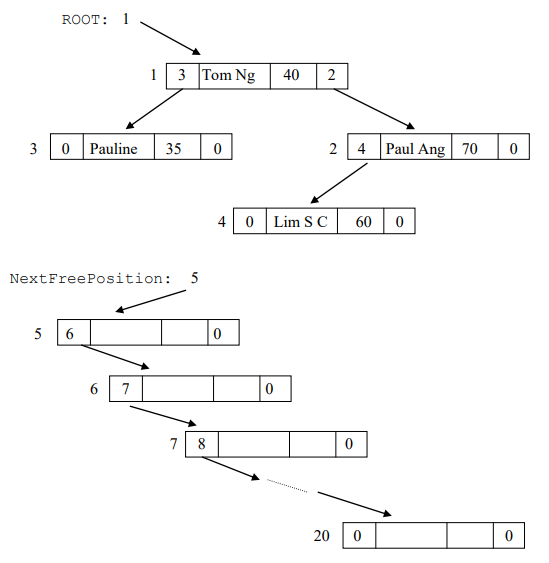
\includegraphics[width=0.65\paperwidth]{C:/Users/Admin/Desktop/Github/question_bank/LyX/static/img/9597-HCI-2015-P1-Q4-1}
\par\end{center}

The diagram shows the binary tree with the students\textquoteright{}
scores 40, 70, 35 and 60 (added in that order) and linked list of
unused nodes after the four students\textquoteright{} scores have
been added. 

\subsection*{Task 4.1 }

Write the program code to declare all the required variables and create
the initial linked list which contains all 20 nodes. Add statement(s)
to initialize the empty tree. 

\subsection*{Evidence 17: }

Your program code for Task 4.1. {[}8{]} 

The following (incomplete) pseudocode inserts a student\textquoteright s
name and his/her score into the binary tree structure. 

The \texttt{LastMove} variable holds the direction of the previous
traversal move as follows: 

X -{}- no move yet made 

L -{}- move was to the left

R -{}- move was to the right 

\noindent %
\noindent\begin{minipage}[t]{1\columnwidth}%
\texttt{PROCEDURE AddNodeToBinaryTree(NewName, NewScore) \bigskip{}
}

\texttt{IF Root = 0 }

\texttt{\qquad{}THEN }

\texttt{\qquad{}\qquad{}Root <- NextFreePosition }

\texttt{\qquad{}ELSE }

\texttt{\qquad{}\qquad{}//traverse the tree to find the position
for the new value }

\texttt{\qquad{}\qquad{}CurrentPosition <- Root }

\texttt{\qquad{}\qquad{}LastMove <- \textquoteleft X\textquoteright{} }

\texttt{\qquad{}\qquad{}REPEAT}

\texttt{\qquad{}\qquad{}\qquad{}PreviousPosition <- CurrentPosition }

\texttt{\qquad{}\qquad{}\qquad{}IF NewScore < ThisTree{[}CurrentPosition{]}.Score }

\texttt{\qquad{}\qquad{}\qquad{}\qquad{}THEN }

\texttt{\qquad{}\qquad{}\qquad{}\qquad{}\qquad{}//move left }

\texttt{\qquad{}\qquad{}\qquad{}\qquad{}\qquad{}LastMove <- \textquoteleft L\textquoteright{} }

\texttt{\qquad{}\qquad{}\qquad{}\qquad{}\qquad{}CurrentPosition
\textleftarrow{} ThisTree{[}CurrentPosition{]}.LeftP }

\texttt{\qquad{}\qquad{}\qquad{}\qquad{}ELSE}

\texttt{\qquad{}\qquad{}\qquad{}\qquad{}\qquad{}// move right }

\texttt{\qquad{}\qquad{}\qquad{}\qquad{}\qquad{}LastMove <- \textquoteleft R\textquoteright{} }

\texttt{\qquad{}\qquad{}\qquad{}\qquad{}\qquad{}CurrentPosition
\textleftarrow{} ThisTree{[}CurrentPosition{]}.RightP }

\texttt{\qquad{}\qquad{}\qquad{}ENDIF }

\texttt{\qquad{}UNTIL CurrentPosition = 0}

\texttt{ENDIF \bigskip{}
}

\texttt{IF LastMove = \textquoteleft R\textquoteright{} }

\texttt{\qquad{}THEN }

\texttt{\qquad{}\qquad{}ThisTree{[}PreviousPosition{]}.RightP <-
NextFreePosition }

\texttt{\qquad{}ELSE }

\texttt{\qquad{}\qquad{}ThisTree{[}PreviousPosition{]}.LeftP <-
NextFreePosition}

\texttt{ENDIF }

\texttt{NextFreePosition \textleftarrow{} ThisTree{[}NextFreePosition{]}.LeftP\bigskip{}
}

\texttt{ENDPROCEDURE }%
\end{minipage}

Note: The above text is available in the text file \texttt{PSEUDOCODE\_TASK\_4\_2.txt} 

\subsection*{Task 4.2 }

Write non-recursive code to implement the \texttt{AddNodeToBinaryTree}
procedure that will add a new node with student\textquoteright s name
and score into the binary tree structure. 

You may use the text file \texttt{PSEUDOCODE\_TASK\_4\_2.txt} as a
basis for the writing of your code. 

The given pseudocode is incomplete as: 
\begin{itemize}
\item it does not initially test that there is free node available for a
new student 
\item it does not assign \texttt{NewName} and \texttt{NewScore} to the data
fields of the \texttt{ThisTree} array Add these requirements to your
program solution.
\end{itemize}

\subsection*{Evidence 18: }

Your program code for Task 4.2. \hfill{} {[}6{]}

\subsection*{Task 4.3 }

Write a procedure \texttt{OutputData} which displays the value of
\texttt{Root}, the value of \texttt{NextFreePosition} and the contents
of \texttt{ThisTree} in index order.

\subsection*{Evidence 19: }

Your program code for Task 4.3. \hfill{}{[}5{]}

\subsection*{Task 4.4 }

Write a main program to: construct a binary search tree using the
data provided in the text file \texttt{SCORES.txt} by calling procedure
\texttt{AddNodeToBinaryTree} . Your program will then call procedure
\texttt{OutputData}. 

\subsection*{Evidence 20: }

Your program code for Task 4.4. \hfill{}{[}3{]}

\subsection*{Evidence 21:}

Screenshot showing the output from running the program in Task 4.4
\hfill{}{[}5{]}

\subsection*{Task 4.5 }

Write a recursive procedure \texttt{RankList} to output the students\textquoteright{}
names and scores in descending scores order. Include a call to the
procedure from your main program. Evidence 22: Your program code for
Task 4.5. {[}6{]} 

\subsection*{Evidence 23: }

Provide a screenshot showing students\textquoteright{} names and scores
in descending scores order. \hfill{} {[}2{]}

{[}SPLIT\_HERE{]}
\item \textbf{{[}HCI/PRELIM/9597/2015/P2/Q1{]} }
\begin{enumerate}
\item What do you understand by the usability of a user interface?\hfill{}
{[}3{]}
\item Handheld mobile devices have become increasing prevalent. Shneiderman\textquoteright s
\textquotedblleft Golden Rules of Interface Design\textquotedblright{}
have existed for some time now. Making use of the \textquotedblleft Golden
Rules\textquotedblright{} as a starting point, grounded in previous
research studies proposes a set of guidelines for mobile device interface
design. Clear explanation needed to articulate your guidelines. Use
examples if necessary to illustrate your point.\hfill{} {[}9{]}
\end{enumerate}
{[}SPLIT\_HERE{]}
\item \textbf{{[}HCI/PRELIM/9597/2015/P2/Q2{]} }
\begin{enumerate}
\item What are the characteristics of client-server network architecture?
\hfill{}{[}2{]} 
\item Give 2 examples of servers and explain how they function in a network.\hfill{}{[}4{]} 
\item Describe how parity bits are used to check the accuracy of a block
of bits. Give an example to support your answers. \hfill{}{[}4{]} 
\item Explain the following cloud computing concepts: 
\begin{enumerate}
\item Software as a service \hfill{}{[}1{]}
\item Platform as a service \hfill{}{[}1{]}
\item Infrastructure as a service \hfill{}{[}1{]}
\end{enumerate}
\end{enumerate}
{[}SPLIT\_HERE{]}
\item \textbf{{[}HCI/PRELIM/9597/2015/P2/Q3{]} }

Your company is starting the development of relational database for
a patient billing system to be marketed to private medical practices
in Singapore. The system is to be called PATMAN (short for PATient
billing MANager), and is to run as a remote client-server system and
a local area network. 

An initial analysis phase of the project has resulted in the following
description of the relevant data for PATMAN. 
\begin{itemize}
\item A practice has a number of patients and doctors. 
\item Doctors are identified by name.
\item Each patient has a number used to identify the patient called the
OHIP number, a name and an age.
\item Each patient is either a male or female and has a next of kin identified
by name.
\item Each medical procedure paid by the government of Singapore is identified
by a procedure code and has a description and a charging category.
\item Each charging category has a dollar value. 
\item Each patient has a number of billing records, with each billing record
recording the medical procedure, the date on which the procedure was
performed, the examining doctor and some additional comments on the
part of the examining doctor.
\item Billing records are either outstanding or paid in full.
\end{itemize}
\begin{enumerate}
\item Draw an ER diagram that represents the PATMAN data. \hfill{}{[}6{]}
\item Using shorthand notation, what are tables in this relational database?\hfill{}
{[}12{]}
\item Explain why relational database is better than a flat file design?\hfill{}
{[}2{]}
\end{enumerate}
{[}SPLIT\_HERE{]}
\item \textbf{{[}HCI/PRELIM/9597/2015/P2/Q4{]} }

The University bookstore sells books online and charges for delivery.
Its delivery charges for orders less than \$200 are as follows: 
\begin{itemize}
\item If the number of items is 3 or less, delivery by next day will be
charged at \$30, while standard delivery will be charged at \$2 per
item. 
\item If the number of items is 4 or more, delivery by next day will be
charged at \$5 per item, while standard delivery is free. 
\end{itemize}
For orders more than \$200, standard delivery is free for any number
of items, while delivery by next day will be charged at \$5 per item. 
\begin{enumerate}
\item Draw a decision table showing all the possible conditions and actions. 
\item Simplify your decision table by removing the redundancies. \hfill{}{[}5{]}
\end{enumerate}
{[}SPLIT\_HERE{]}
\item \textbf{{[}HCI/PRELIM/9597/2015/P2/Q5{]} }

HC university has various campuses around the city and Wilson Parking
is responsible for all the university car parks.

At each car park:

A car arriving triggers a sensor (S1) and a fixed fee (F) is paid
into a machine. This allows a barrier (B1) to be lifted and the car
to enter the car park. When a car leaves the car park it passes over
another sensor (S2) and another barrier (B2) is lifted. 

Each car park has a maximum number of spaces for cars (M) and when
this maximum is reached a \textquotedblleft FULL\textquotedblright{}
sign is illuminated at the entrance and the barrier (B1) will not
rise. The car park is closed at least once a day for cleaning purposes. 
\begin{enumerate}
\item Write an algorithm which will control the barriers and which will
keep a total (T) of the fees paid. \hfill{}{[}8{]}

There are 100 car parks, each of which is identified by a number between
1 and 100. 

At the end of each month, the total fees paid for that month (T) is
collected from each of the car parks as an integer value. 

All data are stored in an array Parks(). 
\begin{itemize}
\item For car park x, Parks(x, 1) to Parks(x, 12) contains the totals for
the twelve months of the year.
\item Parks(x, 13) contain the annual total fees collected for each car
park.
\end{itemize}
\item Using Parks(x,y) to identify individual values in the array, write
an algorithm which can be used to produce the annual totals once the
twelve monthly totals have been input to the array, and the grand
annual total for all the 100 carparks. \hfill{}{[}5{]}
\item When implementing the algorithm into program code, they should be
written to display clarity. Describe \textbf{three} features of the
final program code for this implementation that would achieve this
goal. \hfill{}{[}3{]}
\end{enumerate}
{[}SPLIT\_HERE{]}
\item \textbf{{[}HCI/PRELIM/9597/2015/P2/Q6{]} }

A systems analyst is developing a new computerized admission system
for HC University. 

The project manager identifies the following activities with their
durations and precedence relations: 
\noindent \begin{center}
\begin{tabular}{|c|c|c|}
\hline 
Task & Predecessors & Time(Weeks)\tabularnewline
\hline 
A & - & 3\tabularnewline
\hline 
B & - & 5\tabularnewline
\hline 
C & - & 7\tabularnewline
\hline 
D & A & 8\tabularnewline
\hline 
E & B & 5\tabularnewline
\hline 
F & C & 5\tabularnewline
\hline 
G & E & 4\tabularnewline
\hline 
H & F & 5\tabularnewline
\hline 
I & D & 6\tabularnewline
\hline 
J & G, H & 4\tabularnewline
\hline 
\end{tabular}
\par\end{center}
\begin{enumerate}
\item {}
\begin{enumerate}
\item Draw a Program Evaluation and Review Technique (PERT) chart, show
clearly the early start and late start time of each task, showing
dummy tasks, where necessary. \hfill{}{[}4{]}
\item Explain dependent stages and concurrent stages, giving examples from
your chart. \hfill{}{[}2{]}
\item State the critical path and the minimum time in which the project
can be completed. \hfill{}{[}2{]}
\end{enumerate}
\item Produce a Gantt chart based on the above information. \hfill{}{[}3{]}
\item Give \textbf{one} reason why a Gantt chart may be preferred over a
PERT chart. \hfill{}{[}1{]}
\end{enumerate}
In the current system,
\begin{itemize}
\item Each new student sends a completed form that has their name, date
of birth and the courses that they wish to enroll on. 
\item The date of birth is checked to see whether the student is of the
correct age range for admission to the college. 
\item If the student is too young or too old, a standard rejection letter
is produced. 
\item If the student is of the correct age then each of the courses that
the student has identified are checked on the course file to see whether
they are full or not. 
\item If there is room on a course then the student name is added to the
appropriate course record on the course file. 
\item A standard letter is produced with details of which course(s) the
student has been enrolled on. 
\end{itemize}
\begin{enumerate}
\item[(d)]  
\begin{enumerate}
\item Draw a data flow diagram (DFD) for the current system. \hfill{}{[}6{]}
\item Using examples from your DFD, explain how the diagram helps to inform
a database solution for the new computerized system. \hfill{}{[}4{]}
\item Give \textbf{two} parts of the database design that is not possible
from the DFD. \hfill{}{[}2{]}
\end{enumerate}
\end{enumerate}
{[}SPLIT\_HERE{]}
\item \textbf{{[}HCI/PRELIM/9597/2015/P2/Q7{]} }

Hash table has an index range of 1 to 400. The following pseudocode
describes an algorithm for searching the table using a hashing method.
It is assumed that the key is present in the table. 

\noindent\begin{minipage}[t]{1\columnwidth}%
\texttt{1. index = hash(key)}

\texttt{2. while table(index, 1) <> key }

\texttt{3. \qquad{}index = index + 1}

\texttt{4. endwhile }

\texttt{5. value = table(index, 2) }%
\end{minipage}
\begin{enumerate}
\item Explain the purpose of: 
\begin{enumerate}
\item line 1 
\item line 2 
\item line 3 
\item line 5 
\end{enumerate}
in this algorithm. \hfill{} {[}8{]}
\item The algorithm fails to handle the upper limit on the range of the
index. What modification to the algorithm is required to overcome
this problem? \hfill{} {[}2{]}
\end{enumerate}
{[}SPLIT\_HERE{]}
\end{enumerate}
 
\end{document}
